 %%%%%%%%%%%%%%%%%%%%%%%%%%%%%%%%%%%%%%%%%%%%%%%%%%%%%%%
% A template for Wiley article submissions to Networks.
% Developed by Overleaf.
%
% Modified by D. Shier  (13 Feb 2019)
%%
% Usage notes:
% % Use "num-refs" option for numerical citation and references style.
% % Use the attached wiley-networks.cls and abbrv_networks.bst files.

\documentclass[num-refs]{wiley-networks}

% Add additional packages here if required
\usepackage{graphicx}
\usepackage{caption}
\usepackage{subcaption}

\graphicspath{ {./Figs/} }

% Update article type if known
\papertype{Original Article}
\paperfield{Subsurface Modeling} 

\title{Discontinuous boundary element method for porous media flow problem in 3D discrete fracture networks}

% Use the \authfn to add symbols for additional footnotes and present addresses, if any. Usually start with 1 for notes about author contributions; then continuing with 2 etc if any author has a different present address.

%\author[1\authfn{1}]{Bin Wang}
%\author[2\authfn{2}]{Yin Feng*}
%\author[3\authfn{3}]{Stefano Berrone}
%\author[3]{Sandra Pieraccini}
%\author[3]{Stefano Scial\`o}
%\author[4]{Corrado Fidelibus}
%\author[1\authfn{1}]{Xu Zhou}

\author[1,2]{Bin Wang}
\author[1]{Yin Feng*}
\author[3]{Stefano Berrone}
\author[4]{Sandra Pieraccini}
\author[3]{Stefano Scial\`o}
\author[5]{Corrado Fidelibus}
\author[2]{Xu Zhou}

%\contrib[\authfn{1}]{Equally contributing authors.}


% Include full affiliation details for all authors
\affil[1]{Department of Petroleum Engineering, University of Louisiana at Lafayette, Lafayette, Louisiana, USA}
\affil[2]{Craft \& Hawkins Department of Petroleum Engineering, Louisiana State University, Baton Rouge, LA, USA}
\affil[3]{Dipartimento di Scienze Matematiche, Politecnico di Torino, Torino, Italy}
\affil[4]{Dipartimento di Ingegneria Meccanica e Aerospaziale, Politecnico di Torino, Torino, Italy}
\affil[5]{Dipartimento di Ingegneria dell'Innovazione, Universit\`{a} del Salento, Lecce, Italy}

\corraddress{*Yin Feng, Department of Petroleum Engineering, University of Louisiana at Lafayette}
\corremail{yin.feng@louisiana.edu}


%\presentadd[\authfn{2}]{NA}

\fundinginfo{Funder One, Board of Regents of the State of Louisiana, Grant/Award Numbers: LEQSF(2017-20)-RD-A-20; Funder Two, Funder Two Department, Grant/Award Number: 123459}

% Include the name of the author that should appear in the running header
\runningauthor{Author One et al.}


\begin{document}

\maketitle

\begin{abstract}
Modeling subsurface flow in three-dimensional (3D) discrete fracture networks (DFNs) is of interest of many engineering problems, such as natural gas production and geothermal energy extractions. However, the recent grid-based models are still suffering from the complex gridding issue and high computational burden. In this work, a meshless boundary element method (BEM) approach is presented for the flow in DFNs with arbitrary geometries and penetrated wellbores.
A DFN consists of planar polygonal fractures with random orientation, size and flow transmissivity. Based ...
The presented method is verified against a commercial finite element method (FEM) simulator on several synthetic ... 

Source code is available at 

\textsf{https://github.com/BinWang0213/PyDFN3D}.



% Please include a minimum of six keywords
\keywords{keyword 1, keyword 2, keyword 3, keyword 4, keyword 5}
\end{abstract}

%----------------------------Section 1----------------------------

\section{Introduction}
Please lay out your article using the section headings and example objects below, and remember to delete all help text prior to submitting your article to the journal.

\begin{figure}[h!]
\centering
\includegraphics[width=0.4\textwidth]{ComplexDFN.png}
\caption{Typical DFN problem in engineering application}
\label{fig:DFNs}
\end{figure}

%----------------------------Section 2----------------------------
\section{BEM formulations}
Please lay out your article using the section headings and example objects below, and remember to delete all help text prior to submitting your article to the journal.

%\subsection{Boundary integral equations}
\subsection{Boundary integral equations}
Consider a arbitrary fracture domain $\Omega$ which contains fracture intersections, or traces, $S_{t}$ and wellbore intersections $W_{q}$. The boundary of the domain $\varGamma =\varGamma_\mathrm{D}\cup\varGamma_\mathrm{N}$. $\varGamma_\mathrm{D}$ is the boundary where Dirichlet boundary conditions are prescribed (known as pressure $p$). $\varGamma_\mathrm{N}$ is the boundary where Neumann boundary conditions are prescribed (known as flux $q$). Assuming the fluid viscosity $\mu$ and fracture permeability $k$ is constant over a fracture domain. The governing equation for a steady-state porous media flow in fracture plane containing traces and wellbore intersections can be expressed as follows:
\begin{equation}
    -\nabla \cdot \left( \frac{k}{\mu}\nabla p \right) =q_t+q_s
\label{eq:Laplace}
\end{equation}
Equation~\eqref{eq:Laplace} can be written in integral form, which known as boundary integral equation (BIE), as follows:
\begin{equation}
    -\frac{k}{\mu}\left( c\left( \mathbf{x}_i \right) p\left( \mathbf{x}_i \right) +\int_{\Gamma}{p\left( \mathbf{x} \right) \frac{\partial w\left( \mathbf{x}_i,\mathbf{x} \right)}{\partial \mathbf{n}}d\Gamma} \right) =-\frac{k}{\mu}\int_{\Gamma}{q\left( \mathbf{x} \right) w\left( \mathbf{x}_i,\mathbf{x} \right) d\Gamma}-q_sw\left( \mathbf{x}_i,\mathbf{x} \right) -\int_{S_t}{q_t\left( \mathbf{x} \right) w\left( \mathbf{x}_i,\mathbf{x} \right) dS}
\label{eq:BEM_core}
\end{equation}

The corresponding velocity component $\mathbf{u}\left( u_x,u_y \right)$ BIEs are:
\begin{eqnarray}
    c\left( \mathbf{x}_i \right) u_x\left( \mathbf{x}_i \right) -\frac{k}{\mu}\int_{\Gamma}{p\left( \mathbf{x} \right) \frac{\partial}{\partial x}\left( \frac{\partial w\left( \mathbf{x}_i,\mathbf{x} \right)}{\partial \mathbf{n}} \right) d\Gamma}=-\frac{k}{\mu}\int_{\Gamma}{q\left( \mathbf{x} \right) \frac{\partial w\left( \mathbf{x}_i,\mathbf{x} \right)}{\partial x}d\Gamma}
    %\\
    -q_s\frac{\partial w\left( \mathbf{x}_i,\mathbf{x} \right)}{\partial x}-\int_{S_t}{q_t\left( \mathbf{x} \right) \frac{\partial w\left( \mathbf{x}_i,\mathbf{x} \right)}{\partial x}dS}
    \\
    c\left( \mathbf{x}_i \right) u_y\left( \mathbf{x}_i \right) -\frac{k}{\mu}\int_{\Gamma}{p\left( \mathbf{x} \right) \frac{\partial}{\partial y}\left( \frac{\partial w\left( \mathbf{x}_i,\mathbf{x} \right)}{\partial \mathbf{n}} \right) d\Gamma}=-\frac{k}{\mu}\int_{\Gamma}{q\left( \mathbf{x} \right) \frac{\partial w\left( \mathbf{x}_i,\mathbf{x} \right)}{\partial y}d\Gamma}
    %\\
    -q_s\frac{\partial w\left( \mathbf{x}_i,\mathbf{x} \right)}{\partial y}-\int_{S_t}{q_t\left( \mathbf{x} \right) \frac{\partial w\left( \mathbf{x}_i,\mathbf{x} \right)}{\partial y}dS}
\end{eqnarray}

The detailed derivation of the above BIEs, see Appendix \ref{AppendixA}.

As shown in Fig. \ref{fig:BEM_Nodes}, $\mathbf{x}_i\in \varGamma \cup S\cup T$ a collocation point or source point located on boundaries, traces or wellbores. $\mathbf{x} \in \varGamma \cup S\cup T$ a node point located on the boundaries, traces or wellbores. $p$ is fluid pressure and $q$ is the flux. The fundamental solutions $w$ and $\frac{\partial w}{\partial \mathbf{n}}$ for steady-state porous media flow are \cite{brebbiaBook1994}: 
\begin{eqnarray}
    w\left( \mathbf{x}_i,\mathbf{x} \right) =\frac{1}{2\pi}\ln \frac{1}{r\left( \mathbf{x}_i,\mathbf{x} \right)}
    \\
    \frac{\partial w\left( \mathbf{x}_i,\mathbf{x} \right)}{\partial \mathbf{n}}=\frac{1}{2\pi}\ln \frac{\left( \mathbf{x}_i-\mathbf{x} \right) \cdot \mathbf{n}}{r^2\left( \mathbf{x}_i,\mathbf{x} \right)}
\label{eq:BEM_kernel}
\end{eqnarray}

where $r\left( \mathbf{x}_k,\mathbf{x} \right)$ the distance between $\mathbf{x}_k$ and $\mathbf{x}$.

% subsection{Higher-order discontinuous discretization}
\subsection{Higher-order discontinuous discretization}
In BEM, sets of basis functions is used to discretize the domain boundary and the physical fields. Then, the source point is placed at the collocation points and the BIE in \eqref{eq:BEM_core} is transformed into a system of linear algebraic equations.

Lenti and Fidelibus \cite{lenti2003} proposed a BEM method for DFN where using constant basis functions to deal with the flux discontinuity issue when traces and boundaries intersects each other. However, due to the low accuracy of constant element approximation, it can not handle the complex DFN geometry very well. In this paper, higher-order discontinuous boundary element are used to deal with the flux discontinuity and to achieve high accuracy. As shown in Figs. \ref{fig:BEM_Nodes}-\ref{fig:BEM_Eles}, the fracture boundary $\Gamma$ and traces $S_t$ is discretized by discontinuous quadratic elements. The Wellbore intersection can be accurately represented by exact point source fundamental solution. 

%Figure 2-3
\begin{figure}[h!]
\centering
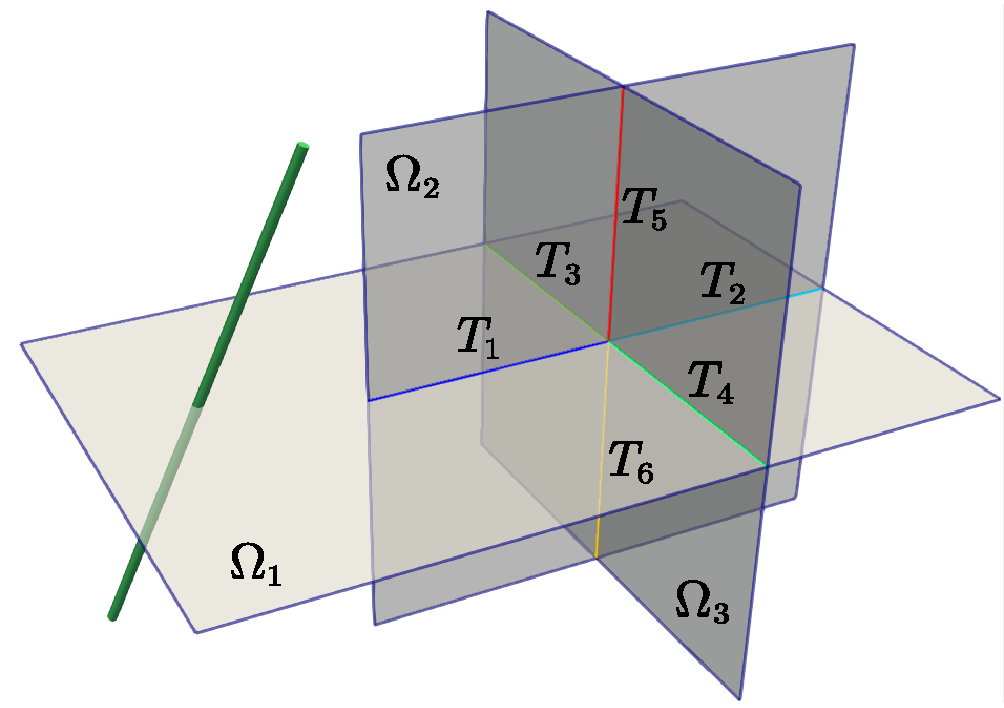
\includegraphics[width=0.3\textwidth]{SimpleDFN.pdf}
\includegraphics[width=0.5\textwidth]{BEM_Mesh.pdf}
\caption{BEM Discretization for a fracture domain, any fracture domain $\Omega$ is considered as a 2D plane. $\mathbf{x}_{i}$ a collocation point or source point. $\mathbf{x}$ is a node point}
\label{fig:BEM_Nodes}
\end{figure}
\begin{figure}[h!]
\centering
\includegraphics[width=0.25\textwidth]{BEM_Element.pdf}
\caption{Discontinues quadratic element used by boundary and trace elements}
\label{fig:BEM_Eles}
\end{figure}

Using the  basis functions, any physical field can be approximated (Fig.\ref{fig:BEM_Eles}) as below:
\begin{equation}
    p\left( \xi \right) =\sum_{k=1}^m{p_k}N _k\left( \xi \right) ,\quad q\left( \xi \right) =\sum_{k=1}^m{q_k}N _k\left( \xi \right) ,\quad -1\leqslant \xi \leqslant 1
\end{equation}

Similarly, the global coordinate system $\mathbf{x}$ can be transformed from local coordinate system $\xi$ by $\mathbf{x}=\sum_{k=1}^N \mathbf{x}_k N_k(\xi)$. $\mathbf{x}_k$ is the coordinate of the collocation points. $p(\mathbf{\xi})$ and $q(\mathbf{\xi})$ now approximations in a finite dimensional space, $p_{k}$, $q_{k}$ unknown nodal values and $\mathbf{N}=\{N_k\}_{k=1,\ldots,m}$ selected basis functions. For the discontinuous quadratic basis functions, the collocation points are shifted inside by an offset $\alpha$ as:
\begin{equation}
    N_1=\frac{1}{2}\frac{\xi}{\alpha}\left( \frac{\xi}{\alpha}-1 \right) , N_2=\left( 1-\frac{\xi}{\alpha} \right) \left( 1+\frac{\xi}{\alpha} \right) , N_3=\frac{1}{2}\frac{\xi}{\alpha}\left( \frac{\xi}{\alpha}+1 \right)
    ,\quad 0.5 < \alpha \leqslant 1
\end{equation}
Substituting the discretized pressure and flux on fracture boundary $\Gamma$, traces $T$ and wellbore intersection $S$ into the BIE \eqref{eq:BEM_core} gives:
\begin{eqnarray}
    c_ip_{i}^{\Gamma}+\sum_{j=1}^{n_{\Gamma}}{H_{ij}^{\Gamma \Gamma}p_{j}^{\Gamma}}=\sum_{j=1}^{n_{\Gamma}}{G_{ij}^{\Gamma \Gamma}q_{j}^{\Gamma}}+\sum_{j=1}^{n_T}{G_{ij}^{\Gamma T}q_{j}^{T}}+\sum_{j=1}^{n_S}{G_{ij}^{\Gamma S}q_{j}^{S}}
    \\
    c_ip_{i}^{T}+\sum_{j=1}^{n_{\Gamma}}{H_{ij}^{T\Gamma}p_{j}^{\Gamma}}=\sum_{j=1}^{n_{\Gamma}}{G_{ij}^{T\Gamma}q_{j}^{\Gamma}}+\sum_{j=1}^{n_T}{G_{ij}^{TT}q_{j}^{T}}+\sum_{j=1}^{n_S}{G_{ij}^{TS}q_{j}^{S}}
    \\
    c_ip_{i}^{S}+\sum_{j=1}^{n_{\Gamma}}{H_{ij}^{S\Gamma}p_{j}^{\Gamma}}=\sum_{j=1}^{n_{\Gamma}}{G_{ij}^{S\Gamma}q_{j}^{\Gamma}}+\sum_{j=1}^{n_T}{G_{ij}^{ST}q_{j}^{T}}+\sum_{j=1}^{n_S}{G_{ij}^{SS}q_{j}^{S}}
\label{eq:BEM_Discretization}
\end{eqnarray}
where the integrals of fundamental solutions are $G=\int_{\Gamma}{w\left( \mathbf{x}_i,\mathbf{x} \right)}\mathbf{N}^Td\Gamma ,H=\int_{\Gamma}{\frac{\partial w\left( \mathbf{x}_i,\mathbf{x} \right)}{\partial \mathbf{n}}}\mathbf{N}^Td\Gamma$. Eq. \eqref{eq:BEM_Discretization} can be expressed as in matrix form:
\begin{equation}
    \left[ \begin{matrix}
    	C^{\Gamma}+H^{\Gamma \Gamma}&		\mathbf{0}&		\mathbf{0}\\
    	H^{T\Gamma}&		C^T&		\mathbf{0}\\
    	H^{S\Gamma}&		\mathbf{0}&		C^S\\
    \end{matrix} \right] \left\{ \begin{array}{c}
    	p^{\Gamma}\\
    	p^T\\
    	p^S\\
    \end{array} \right\} =\left[ \begin{matrix}
    	G^{\Gamma \Gamma}&		G^{\Gamma T}&		G^{\Gamma T}\\
    	G^{T\Gamma}&		G^{TT}&		G^{TS}\\
    	G^{S\Gamma}&		G^{ST}&		G^{SS}\\
    \end{matrix} \right] \left\{ \begin{array}{c}
    	q^{\Gamma}\\
    	q^T\\
    	q^S\\
    \end{array} \right\} 
\end{equation}
where $C$ is the diagonal matrix from the free term $c$ and singular integral values $H$ when source point $\mathbf{x}_i$ and node point $\mathbf{x}$ are overlapped.  

%\subsection{Fast analytical integration}
\subsection{Fast analytical integration}
After BEM discretization, there are singular integration, nearly singular integration and non-singular integration needs to be calculated due to the singularities in fundamental solution and BIEs. The singular integration and nearly singular integration need to be carefully treated in BEM due to the classic numerical integration will lead to large errors \cite{katsikadelisBook2016}. Numerous methods have been developed to integrate singular and nearly singular integration in an efficient manner, and one can refer to \cite{LiuYJBook2006,tanaka1994}. Such as element subdivision, analytical and semi-analytical integration, adaptive Gaussian quadrature, coordinate transformation and BIE modification \cite{gu2016Singular}. Several exact analytical integration formulations developed in \cite{fratantonio2000exact,zhang2003exact,zhang2008exact} which can calculate singular integration terms accurately and efficiently. 

In this paper, the exact integration formulations for discontinuous quadratic element is derived based on the method proposed by \cite{zhang2003exact}. The integrals $G,H$ in Eq.\eqref{eq:BEM_Discretization} can be expressed as:
\begin{eqnarray}
G=\left[ G_1,G_2,G_3 \right] ^T=\int_{\Gamma}{w\left( \mathbf{x}_i,\mathbf{x} \right)}\left[ N_1,N_2,N_3 \right] ^Td\Gamma 
\\
H=\left[ H_1,H_2,H_3 \right] ^T=\int_{\Gamma}{\frac{\partial w\left( \mathbf{x}_i,\mathbf{x} \right)}{\partial \mathbf{n}}}\left[ N_1,N_2,N_3 \right] ^Td\Gamma 
\label{eq:BEM_Integrals}
\end{eqnarray}
When a source point isn't on a boundary element, the analytical integration formulations are:
\begin{eqnarray}
    G_1=\frac{1}{2\pi}\frac{J}{4}\left( \frac{A_2}{\alpha ^2}-\frac{A_1}{\alpha} \right) , G_2=\frac{1}{2\pi}\frac{J}{2}\left( A_0-\frac{A_2}{\alpha ^2} \right) ,G_3=\frac{1}{2\pi}\frac{J}{4}\left( \frac{A_2}{\alpha ^2}+\frac{A_1}{\alpha} \right) 
    \\
    H_1=\frac{1}{2\pi}\frac{e}{2}\left( \frac{F_2}{\alpha ^2}-\frac{F_1}{\alpha} \right) , H_2=\frac{1}{2\pi}e\left( F_0-\frac{F_2}{\alpha ^2} \right) ,H_3=\frac{1}{2\pi}\frac{J}{2}\left( \frac{F_2}{\alpha ^2}+\frac{F_1}{\alpha} \right) 
\label{eq:BEM_ExactInt1}
\end{eqnarray}
When a source point is on a boundary element, the analytical integration formulations are:
\begin{eqnarray}
    &G_1=\frac{1}{2\pi}\frac{J}{2}\left( \frac{S_2}{\alpha ^2}-\frac{S_1}{\alpha} \right) ,G_2=\frac{1}{2\pi}J\left( S_0-\frac{S_2}{\alpha ^2} \right) ,G_3=\frac{1}{2\pi}\frac{J}{2}\left( \frac{S_2}{\alpha ^2}+\frac{S_1}{\alpha} \right) 
    \\
    &H_1=H_2=H_3=0
\label{eq:BEM_ExactInt2}
\end{eqnarray}
where $A,F,S,J,e$ are analytical integration terms are given in Appendix \ref{AppendixB}. 

\subsection{Parallel domain decomposition algorithm}
After BEM discretization, there are singular integration, nearly singular integration and non-singular integration needs to be calculated due to the singularities in fundamental solution and BIEs. The singular integration and nearly singular integration need to be carefully treated in BEM due to the classic numerical integration will lead to large errors \cite{katsikadelisBook2016}.

%----------------------------Section 3----------------------------
\section{Numerical examples}
In this section, numerical examples are presented as follows: In the first example, the proposed algorithm is verified against an exact solution on a unit square fracture with a line source and a point source. In the next two examples, the application of the presented algorithm is demonstrated on two complex DFNs system.  

\subsection{Unit square problem}
The performance of the proposed method is firstly evaluated with a simple problem without traces and sources. Consider the porous media flow in a unit square $\left( x,y \right) \,\,\in \,\,\left( \text{0,}1 \right) \times \left( \text{0,}1 \right), \mu =1, k=1$ with the following the exact solution (Fig. \ref{fig:Case_Exact}):
\begin{equation}
    p\left( x,y \right) =\text{15}\cos \left( 4\pi x \right) \frac{\sinh \left( 4\pi y \right)}{\pi \cosh \left( 4\pi \right)}
\end{equation}
The relative error of the proposed algorithm are quantitatively analyzed by computing L2 norm error for N sampling points over the computation domain as below:
\begin{equation}
    e_p=\sqrt{\frac{\sum_{l=1}^N{\left( p_{l,exact}-p_{l,h} \right) ^2}}{N}}, \quad e_{\mathbf{u}}=\sqrt{\frac{\sum_{l=1}^N{\left( \mathbf{u}_{l,exact}-\mathbf{u}_{l,h} \right) \cdot \left( \mathbf{u}_{l,exact}-\mathbf{u}_{l,h} \right)}}{N}}
\end{equation}
where $N=1600$ sampling points are uniformly distributed over the domain. 

\begin{figure}[h!]
\centering
\includegraphics[width=0.4\textwidth]{UnitSquare.pdf}
\includegraphics[width=0.4\textwidth]{Exact_Field.pdf}
\caption{Unit square problem: $\Omega$ is a unit square with 3 Neumann BCs and 1 Dirichlet BC}
\label{fig:Case_Exact}
\end{figure}

As shown in Fig. \ref{fig:BEM_Convergence}, a reference finite-element-method (FEM) solution (using continuous quadratic element) is compared with BEM solution with constant element, discontinuous linear element and discontinuous quadratic element. Results show that the proposed BEM algorithm is more accurate than FEM, especially for velocity component. Also, higher-order quadratic BEM element is much accurate than the commonly used constant/linear element by 2-4 orders of magnitude.
\begin{figure}[h!]
\centering
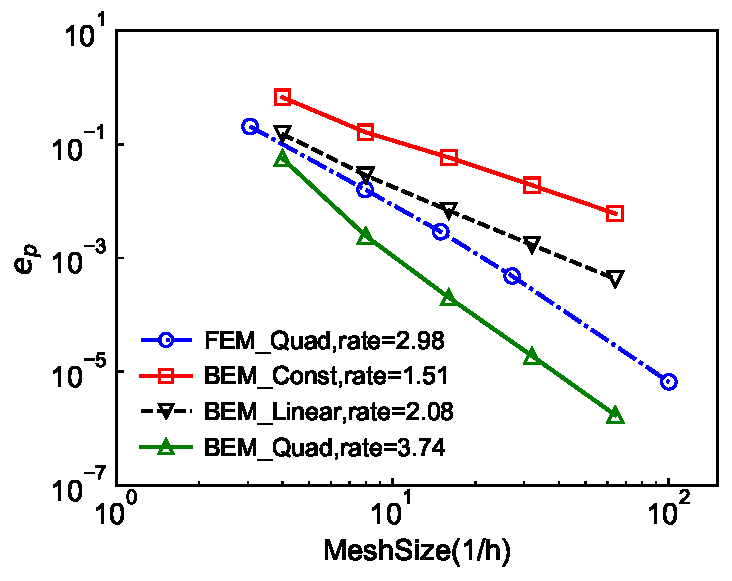
\includegraphics[width=0.45\textwidth]{L2_Pressure.pdf}
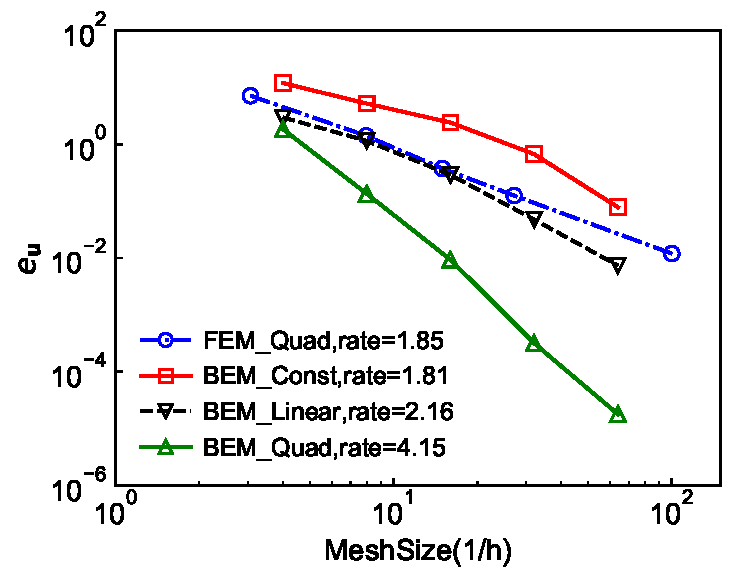
\includegraphics[width=0.45\textwidth]{L2_Velocity.pdf}
\caption{Convergence analysis of BEM solver for pressure $p$ and velocity $\mathbf{u}$ with PyDFN3D }
\label{fig:BEM_Convergence}
\end{figure}

\subsection{Single fracture domain problem}
In order to further evaluate the capabilities and performance of the proposed algorithm, a single fracture domain with one trace and one well is tested. In this problem, trace is uniformly prescribed with pressure of -5 Pa and wellbore is prescribed with pressure 3 Pa. All other parameters are adopted from the example 1. 
\begin{figure}[h!]
\centering
    \includegraphics[width=0.4\textwidth]{UnitSquareTS.pdf}
    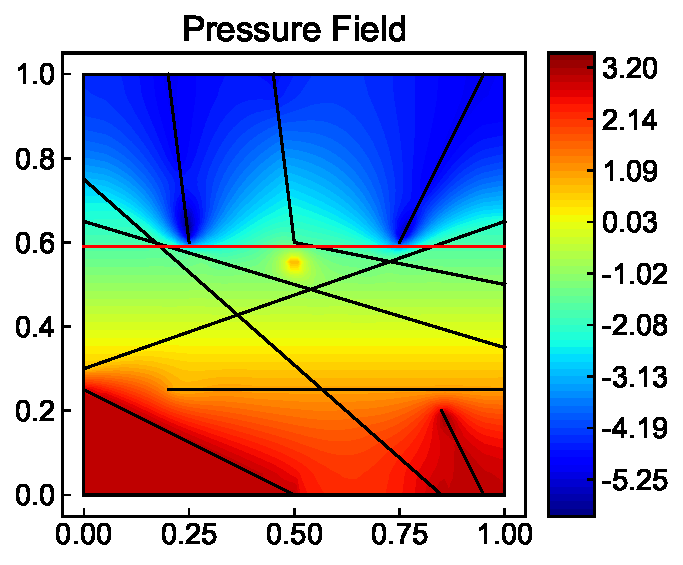
\includegraphics[width=0.4\textwidth]{Case2_Pressure_Field.pdf}
\caption{Single fracture domain problem: $\Omega$ is a unit square with 3 Neumann BCs and 1 Dirichlet BC. Trace is prescribed with pressure of -5 Pa and wellbore is prescribed with pressure of 3 Pa. }
\label{fig:Case2_info}
\end{figure}
\begin{figure}[h!]
\centering
    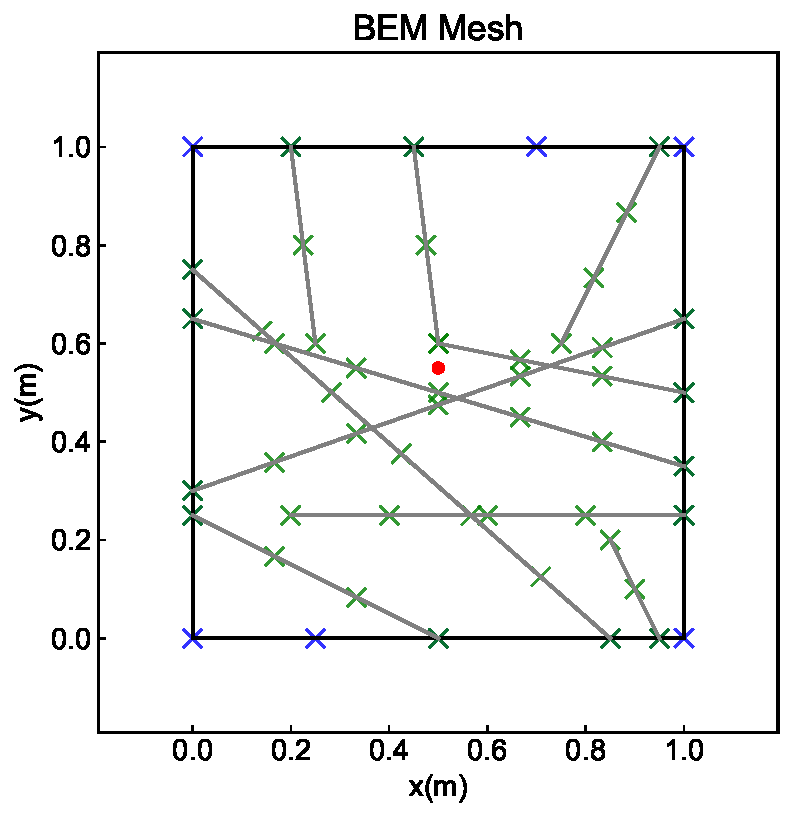
\includegraphics[width=0.3\textwidth]{Case2_BEM_Mesh.pdf}
    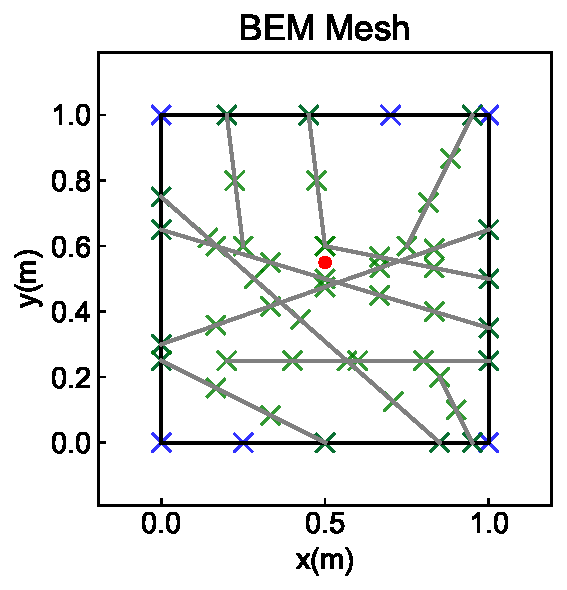
\includegraphics[width=0.3\textwidth]{Case2_BEM_Mesh_refine.pdf}
\vskip\baselineskip
    \includegraphics[width=0.27\textwidth]{Case2_FEM_Mesh_uniformc.png}
    \quad
    \includegraphics[width=0.27\textwidth]{Case2_FEM_Mesh_LGRc.png}
\caption{Comparison of typical meshes for fracture modeling: BEM coarse mesh has 20 elements and refine mesh has 97 elements; FEM uniform mesh has 1924 elements and LGR mesh has 9432 elements}
\label{fig:Case2_Mesh}
\end{figure}

As shown in Figs. \ref{fig:Case2_Mesh}-\ref{fig:Case2_PressureOverLine}, BEM solution with 97 elements has the same level of accuracy in FEM with 9432 elements. Due to the semi-analytical nature of BEM, accurate pressure solution at the wellbore can be achieved with only one nodes. However, locally grid refinement (LGR) has to be applied in FEM. Results show that BEM eliminates the complex meshing issue in FEM and maintains the high solution accuracy.

\begin{figure}[h!]
\caption{Small scale DFNs domain of Case 3, injector $S_{Inj}$ with pressure constrains of 2 MPa and producer $S_{Pro}$ with pressure constrains of 1 MPa}
\centering
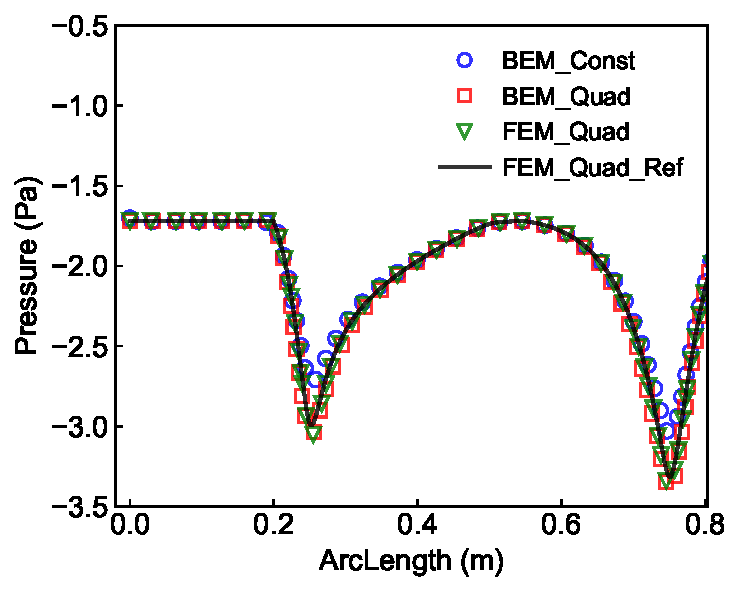
\includegraphics[width=0.5\textwidth]{Case2_PressureOverLine.pdf}
\caption{Comparison of pressure solution on a line of y=0.24 between BEM and FEM; BEM (97 elements) used about 100X less elements than FEM (9432 elements) to achieve the same level of accuracy}
\label{fig:Case2_PressureOverLine}
\end{figure}

\subsection{Four-fracture DFNs problem}
In this example, a simple four rectangle fractures DFNs problem is considered. Three horizontal fractures ,$\Omega_{2-4}$, intersect with 1 vertical fracture, $\Omega_{1}$. One injection well, $S_{Inj}$, penetrates through the fracture,$\Omega_{3}$, and one production well, $S_{Pro}$ penetrates though fractures,$\Omega_{2,4}$, respectively. Pressure boundary conditions are prescribed on injection well and production well, 2 MPa and 1 MPa, respectively. In order to comparing the fully 3D solution with tetrahedron mesh, the aperture of four fractures is set as 0.01 m. Wellbore radius is set as 0.001 m. Fluid viscosity is 0.001 Pa s, fracture permeability is $3\times 10^{-10}\,\,\text{m}^2$.

\begin{figure}
\centering
     \begin{subfigure}[b]{0.45\textwidth}
         \centering
         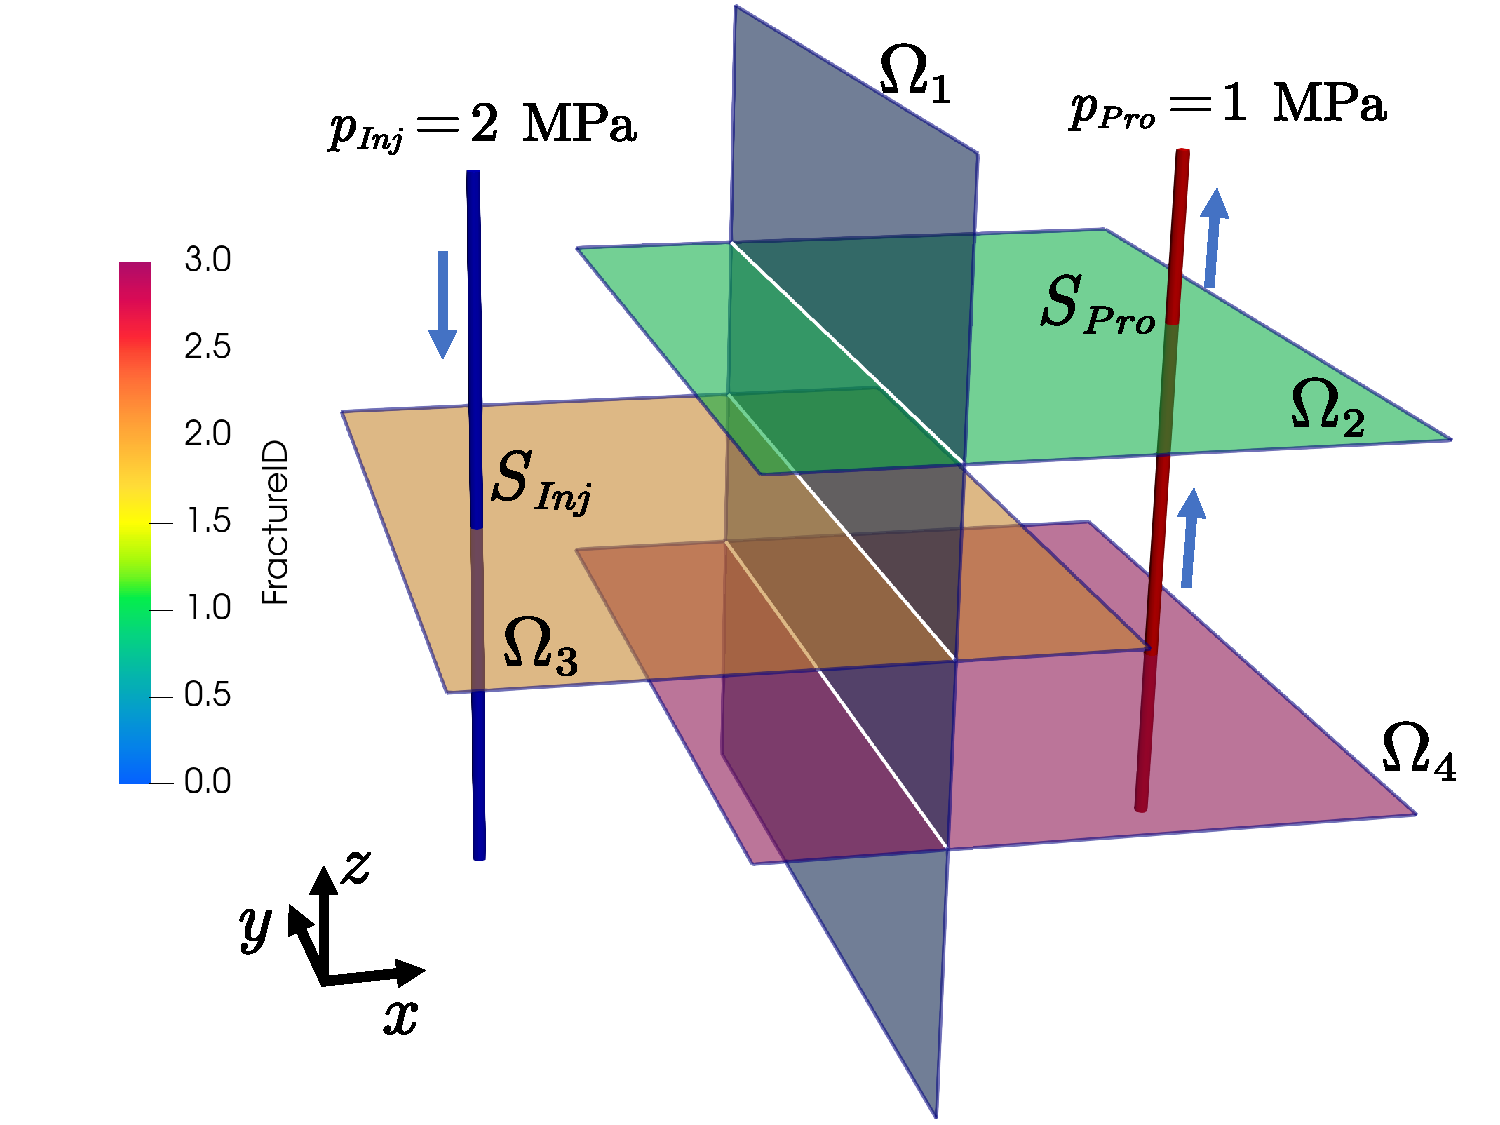
\includegraphics[width=\textwidth]{Case3_Domain.pdf}
         \caption{BEM planar model}
     \end{subfigure}
\quad
     \begin{subfigure}[b]{0.33\textwidth}
         \centering
         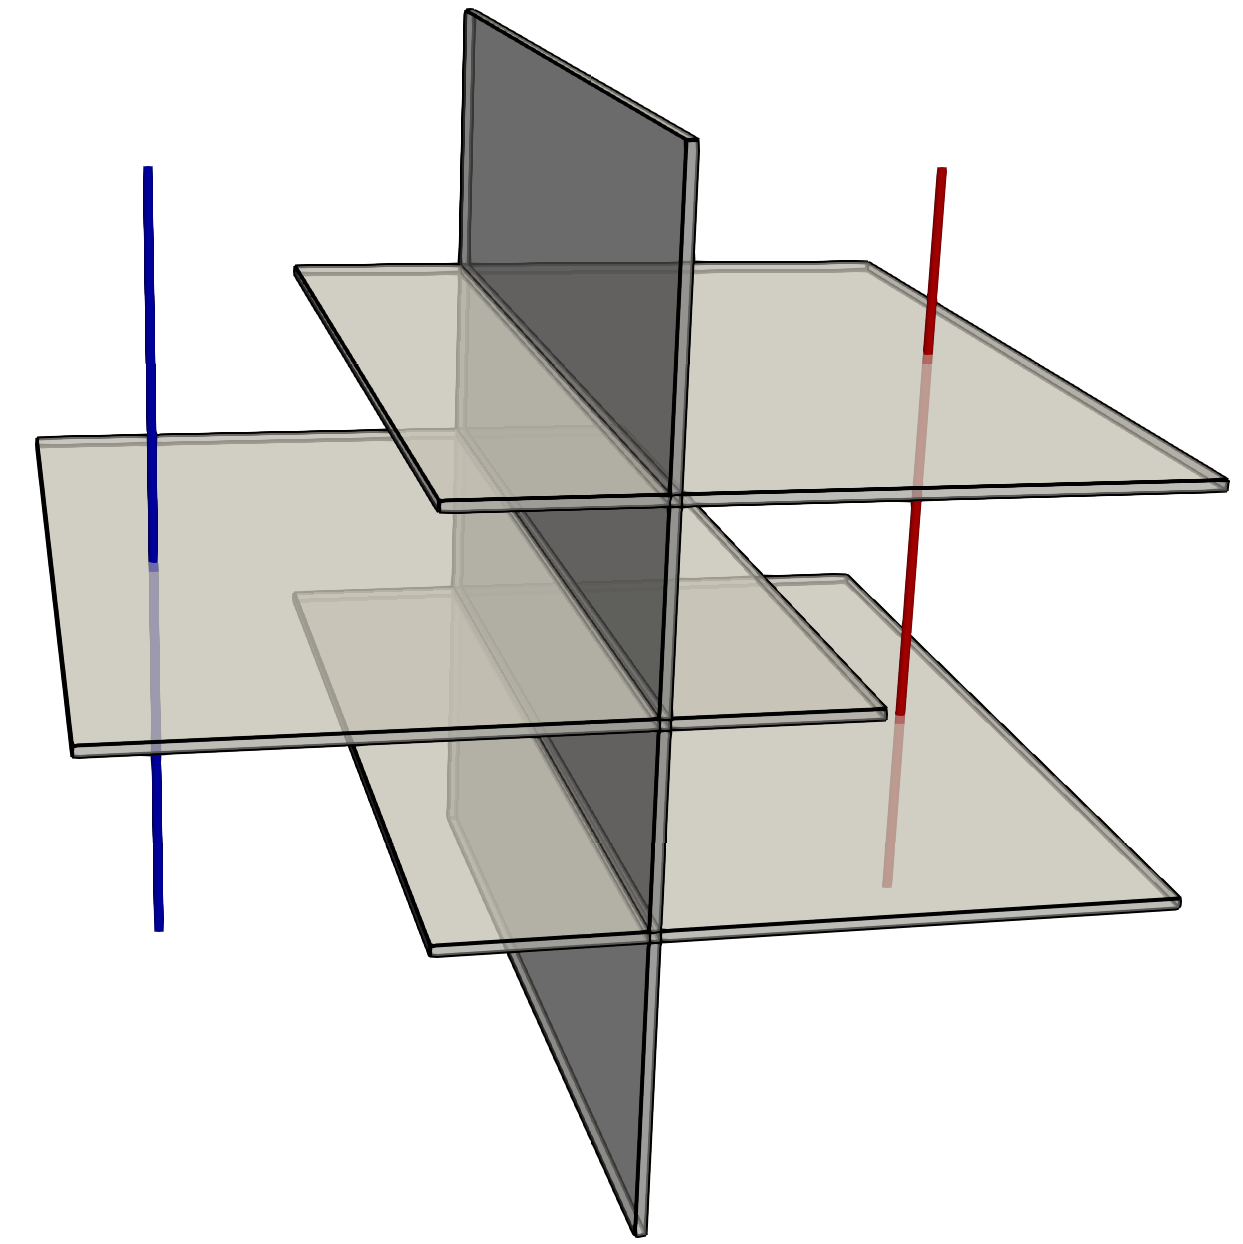
\includegraphics[width=\textwidth]{Case3_FEMDomain_c.png}
         \caption{FEM 3D solid model}
     \end{subfigure}
\label{fig:Case3_Domain}
\caption{DFNs of four fractures. Domain size is $\text{1 m }\times \,\,\text{1 m }\times \,\,\text{1 m }
$. Fracture aperture is constant and equal to 0.01 m. Detailed geometric parameters are shown in \ref{AppendixC}}
\end{figure}

\begin{figure}
\centering
     \begin{subfigure}[b]{0.4\textwidth}
         \centering
         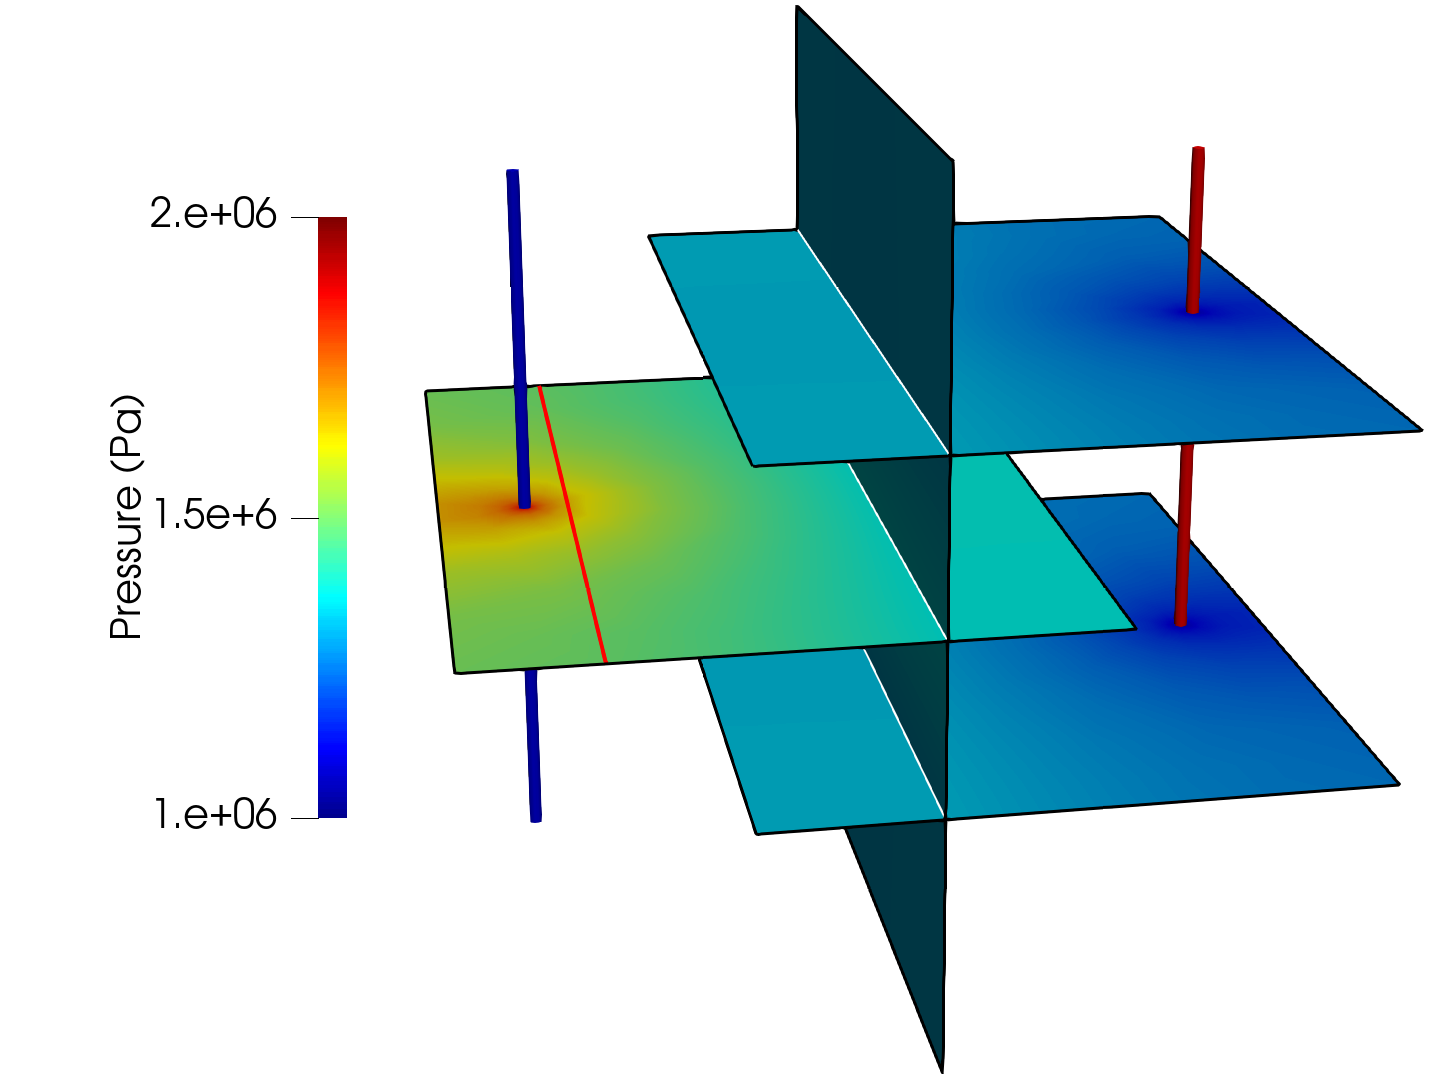
\includegraphics[width=\textwidth]{Case3_pressure_plot.png}
         \caption{Pressure solution contour with a red line}
     \end{subfigure}
\quad
     \begin{subfigure}[b]{0.4\textwidth}
         \centering
         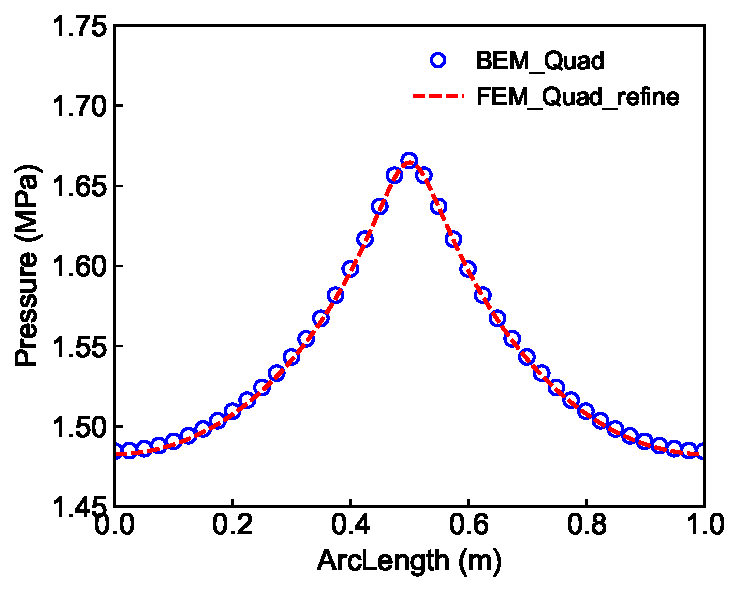
\includegraphics[width=\textwidth]{Case3_PressureOverLine.pdf}
         \caption{Pressure over the red line}
     \end{subfigure}
\vskip\baselineskip
     \begin{subfigure}[b]{0.4\textwidth}
         \centering
         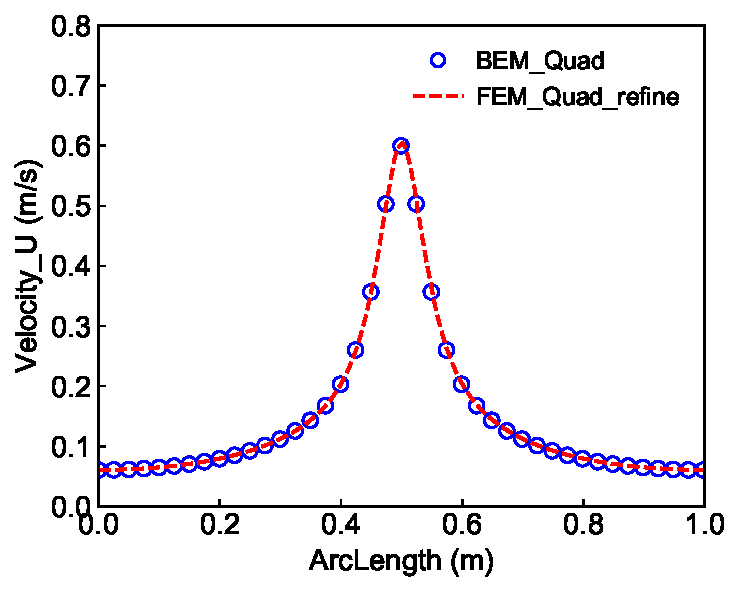
\includegraphics[width=\textwidth]{Case3_VelocityYOverLine_U.pdf}
         \caption{Velocity $u$ over the red line}
     \end{subfigure}
\quad
     \begin{subfigure}[b]{0.4\textwidth}
         \centering
         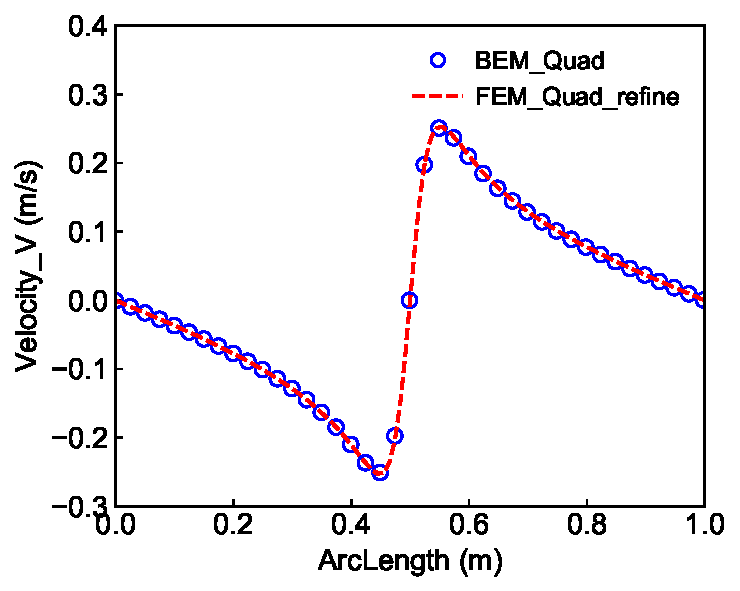
\includegraphics[width=\textwidth]{Case3_VelocityYOverLine_V.pdf}
         \caption{Velocity $v$ over the red line}
     \end{subfigure}
\label{fig:Case3_Solution}
\caption{Pressure and velocity solution of Case 3. Red line in (a) is indicated the line considered for the plots of (b)-(d)}
\end{figure}

\subsection{Synthetic practical problem}
In BEM, sets of basis functions is used to discretize the domain boundary and the physical fields. Then, the source point is placed at the collocation points and the BIE in \eqref{eq:BEM_core} is transformed into a system of linear algebraic equations.

\begin{figure}
\centering
     \begin{subfigure}[b]{0.45\textwidth}
         \centering
         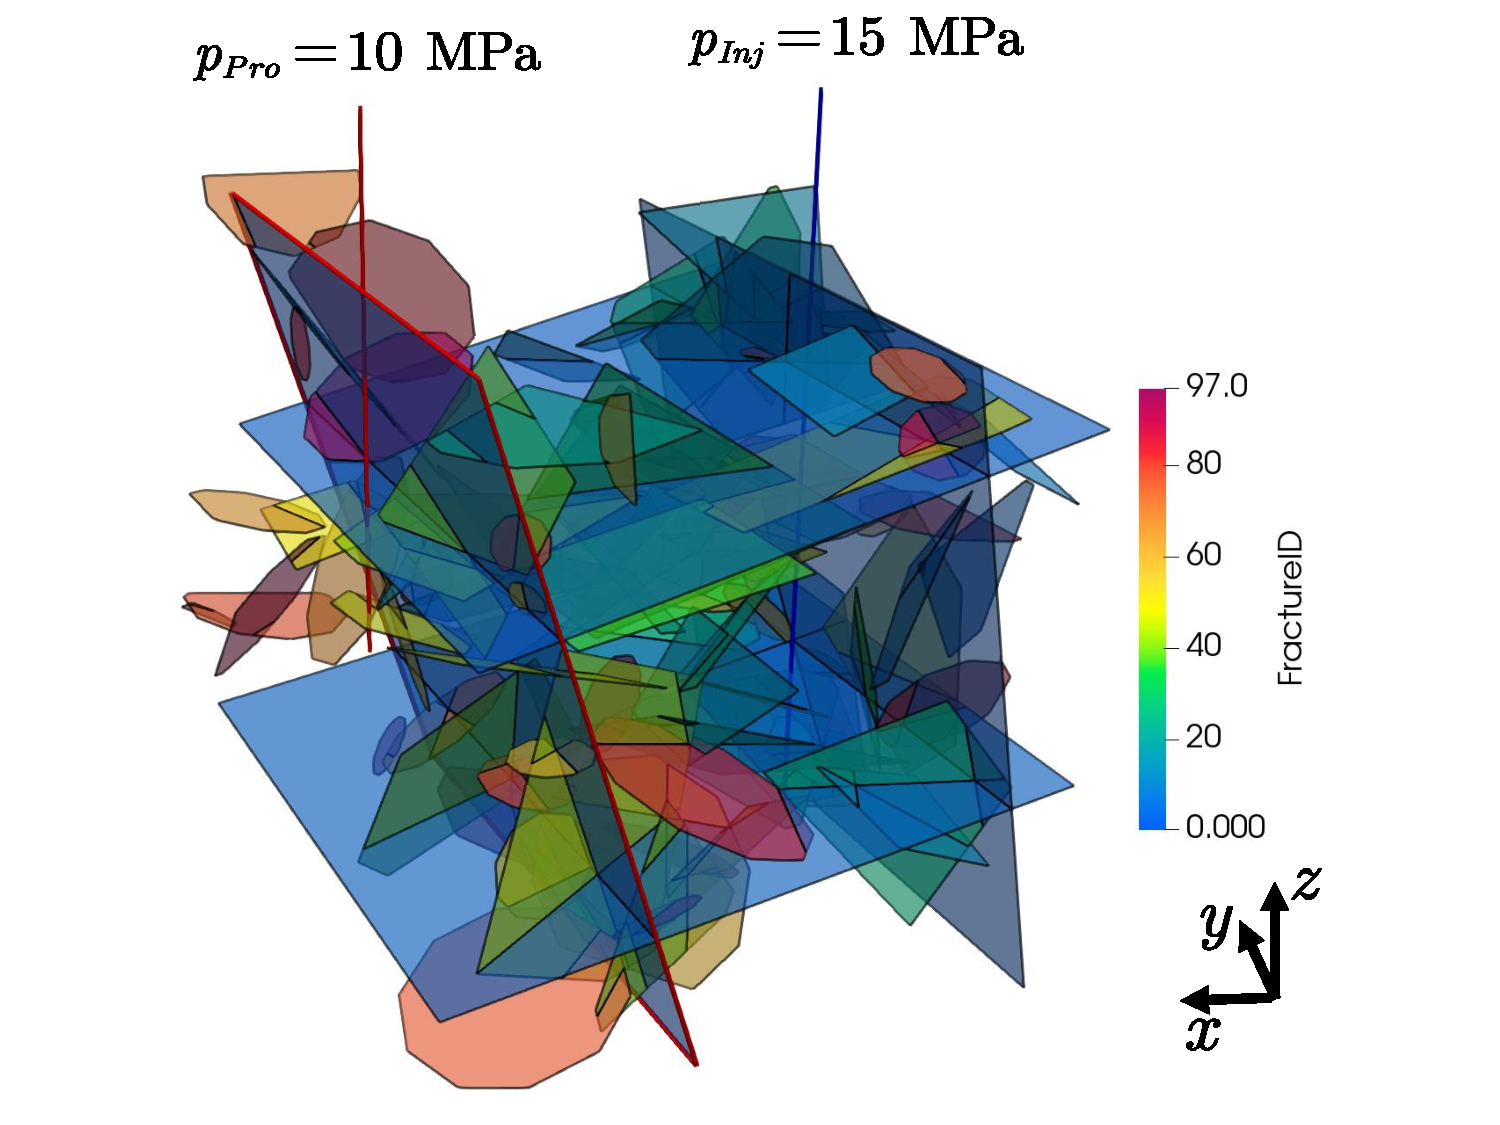
\includegraphics[width=\textwidth]{Case4_Domain.pdf}
         \caption{large scale DFNs model where fracture 0 marked in red}
     \end{subfigure}
\quad
     \begin{subfigure}[b]{0.35\textwidth}
         \centering
         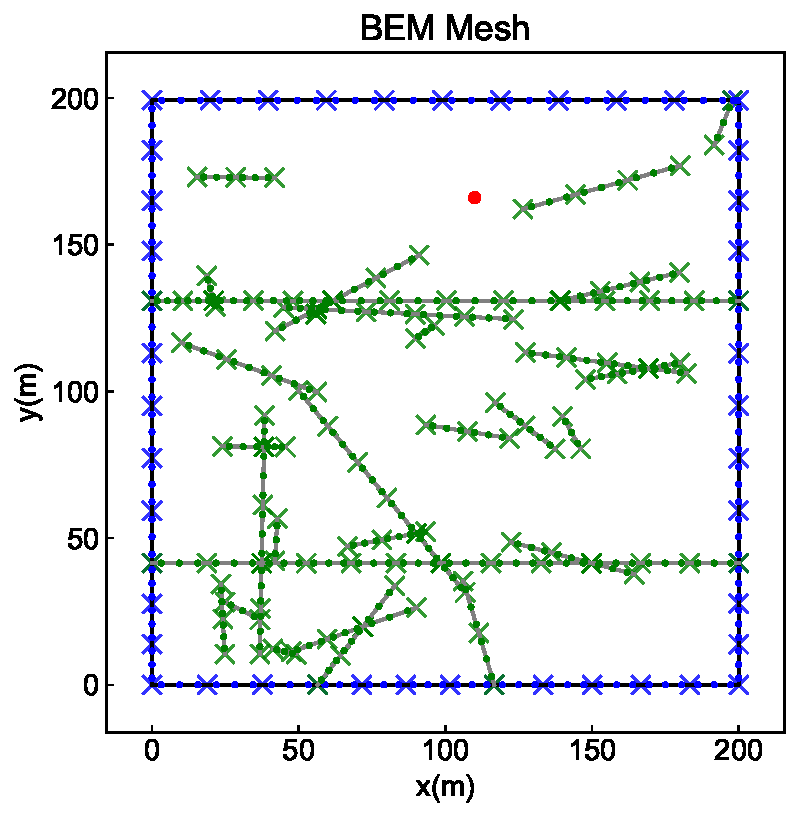
\includegraphics[width=\textwidth]{DFN_Paper/Figs/Case4_BEM_Mesh.pdf}
         \caption{BEM mesh of fracture 0}
     \end{subfigure}
\label{fig:Case4_Domain_Mesh}
\caption{Large scale DFNs probelm of Case 4 with 4 conductive fault and 93 natural fractures, injector $S_{Inj}$ with pressure constrains of 15 MPa and producer $S_{Pro}$ with pressure constrains of 10 MPa}
\end{figure}

\begin{figure}
\centering
     \begin{subfigure}[b]{0.4\textwidth}
         \centering
         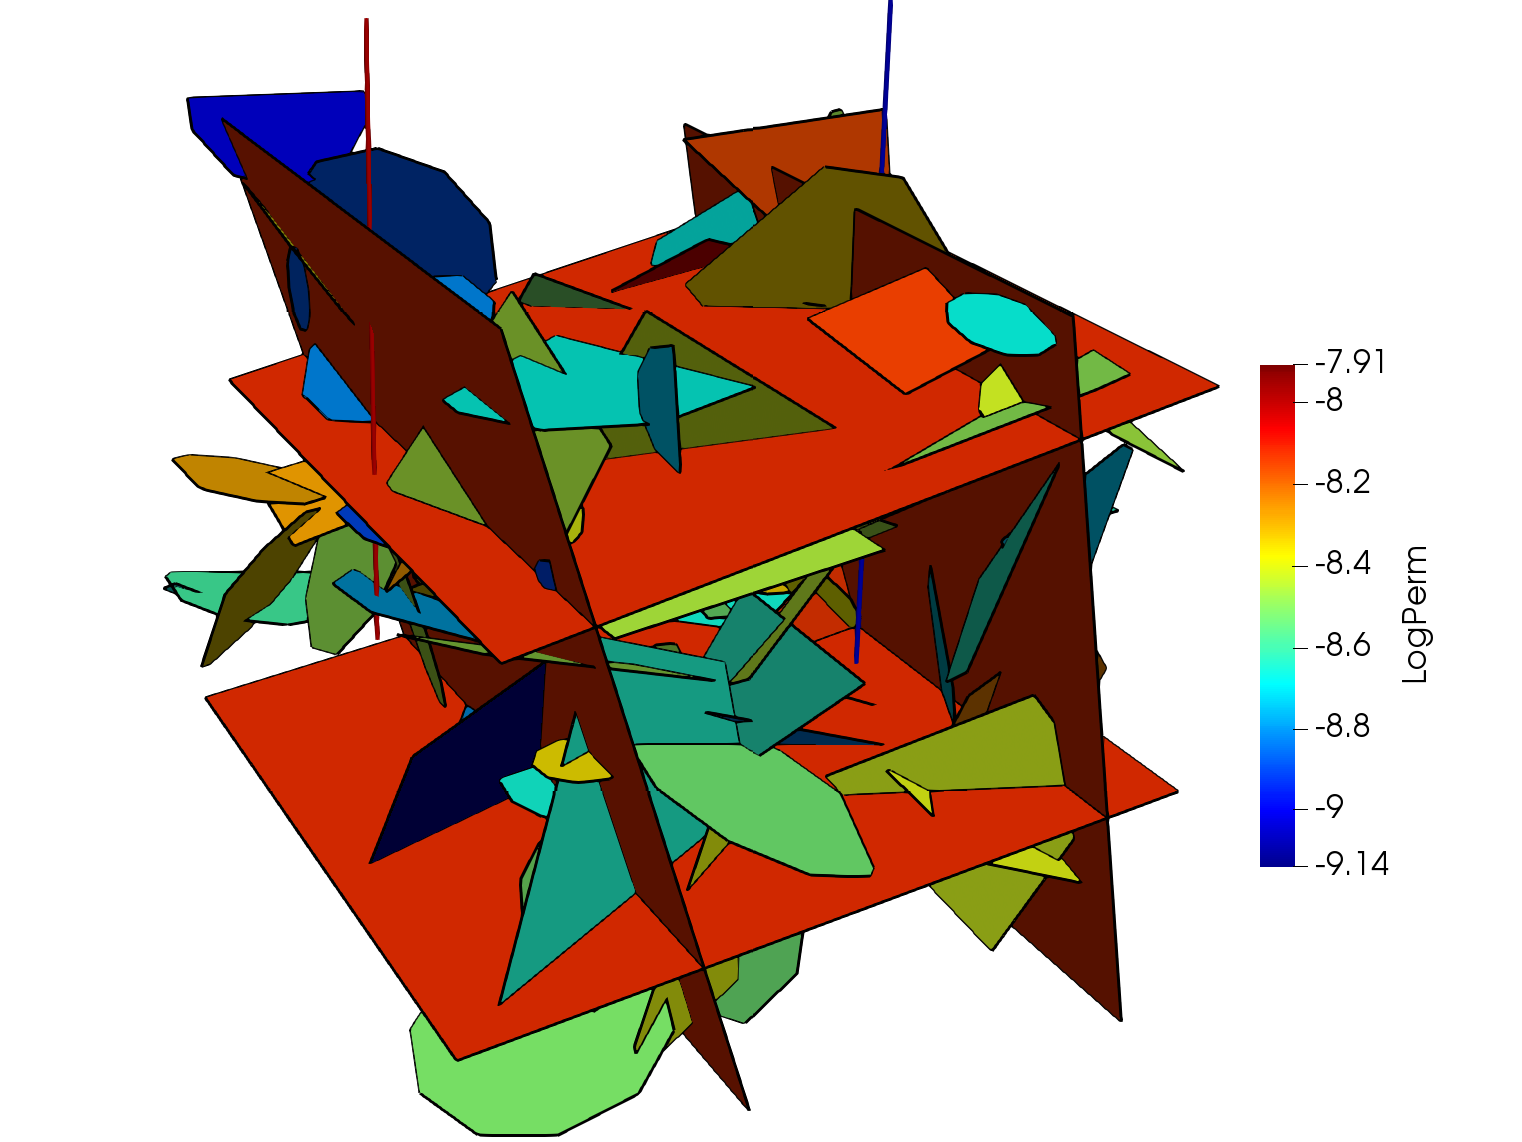
\includegraphics[width=\textwidth]{DFN_Paper/Figs/Case4_LogPerm_c.png}
         \caption{Permeability distribution}
     \end{subfigure}
\quad
     \begin{subfigure}[b]{0.4\textwidth}
         \centering
         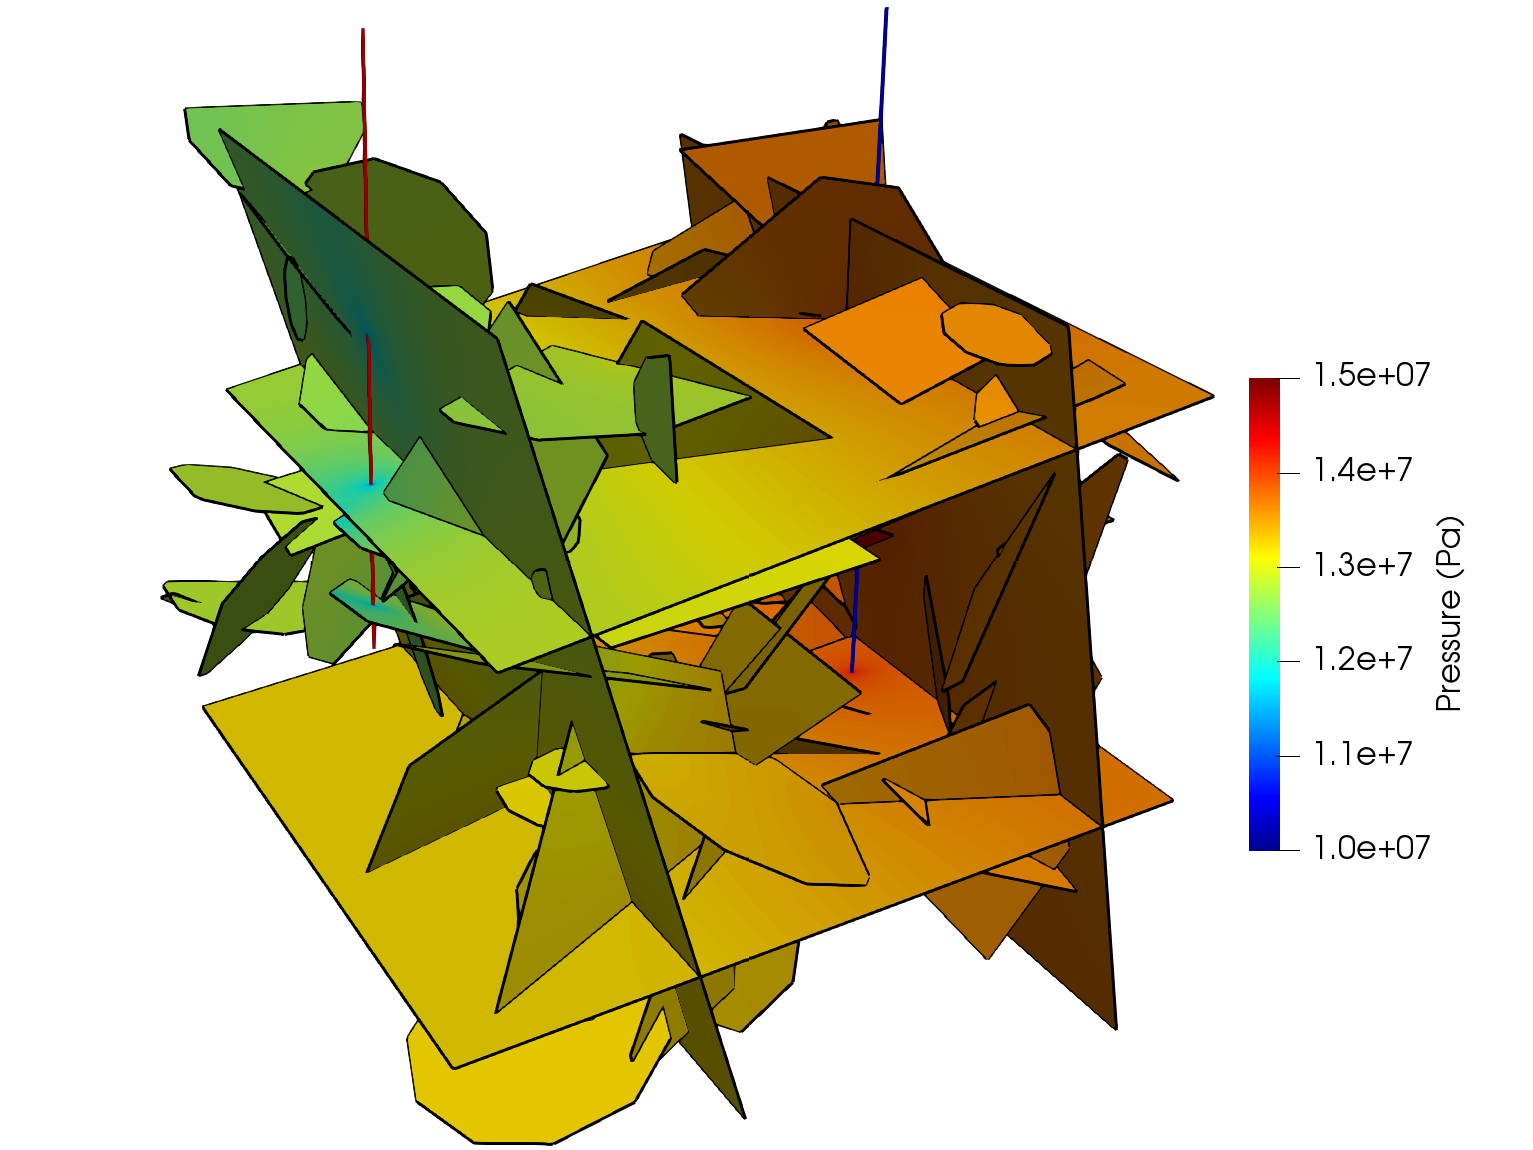
\includegraphics[width=\textwidth]{DFN_Paper/Figs/Case4_Pressure_c.png}
         \caption{Pressure solution}
     \end{subfigure}
\label{fig:Case3_Solution}
\caption{Permeability distribution and pressure solution of Case 4.}
\end{figure}

\section*{\normalsize{ACKNOWLEDGMENTS}}
Acknowledgments should include contributions from anyone who does not meet the criteria for authorship (for example, to recognize contributions from people who provided technical help, collation of data, writing assistance, acquisition of funding, or a department chairperson who provided general support), as well as any funding or other support information.

%REFERENCES
%Note that references are placed in lexicographic order by author name. Multiple entries within a citation should appear in numerical order also, such as [2, 17, 19, 42].

%\bibliographystyle{plain}
\bibliography{sample}


\appendix
\numberwithin{equation}{section} % Renumbering the appendix

%\Appendix A
\section{Derivation of BIEs for porous media flow}
\label{AppendixA}
The governing equation for a steady-state porous media flow can be expressed as follows:
\begin{equation}
-\nabla \cdot \left( \frac{k}{\mu}\nabla p \right) =q
\label{eq:A1}
\end{equation}

Introducing an weighting function $w$, multiply it on the both side of \eqref{eq:A1} and take integration by part, $\int_{\Omega}{\nabla \cdot \left( \nabla pw \right)}d\Omega =\int_{\Omega}{\nabla \cdot \left( \nabla p \right) wd\Omega}+\int_{\Omega}{\nabla p\cdot \nabla wd\Omega}$, gives:
\begin{equation}
    -\frac{k}{\mu}\left( \int_{\Omega}{\nabla \cdot \left( \nabla pw \right)}d\Omega -\int_{\Omega}{\nabla p\cdot \nabla wd\Omega} \right) =\int_{\Omega}{qwd\Omega}
\label{eq:A2}
\end{equation}

Taking integration by part again, $\int_{\Omega}{\nabla \cdot \left( \nabla wp \right)}d\Omega =\int_{\Omega}{\nabla \cdot \left( \nabla w \right) p}d\Omega +\int_{\Omega}{\nabla w\cdot \nabla pd\Omega}$, on the second term of \eqref{eq:A2} gives:
\begin{equation}
    -\frac{k}{\mu}\left( \int_{\Omega}{\nabla \cdot \left( w\nabla p \right)}d\Omega -\int_{\Omega}{\nabla \cdot \left( p\nabla w \right)}d\Omega +\int_{\Omega}{\nabla \cdot \left( \nabla w \right) pd\Omega} \right) =\int_{\Omega}{qwd\Omega}
\label{eq:A3}
\end{equation}

Based on the divergence theorem, $\int_{\Omega}{\nabla \cdot fd\Omega}=\int_{\Gamma}{f\cdot \mathbf{n}d\Gamma}$, the first two terms in \eqref{eq:A3} can be written as boundary integrals as follows:
\begin{equation}
    -\frac{k}{\mu}\left( \int_{\Gamma}{w\nabla p\cdot \mathbf{n} d\Gamma}-\int_{\Gamma}{p\nabla w\cdot \mathbf{n} d\Gamma}+\int_{\Omega}{\nabla \cdot \left( \nabla w \right) p d\Omega} \right) =\int_{\Omega}{q w d\Omega}
\label{eq:A4}
\end{equation}

Based on $\nabla f\cdot\mathbf{n}=\frac{\partial f}{\partial \mathbf{n}}$, \eqref{eq:A4} can be rewritten as follows:
\begin{equation}
    -\frac{k}{\mu}\left( \int_{\Gamma}{w\frac{\partial p}{\partial \mathbf{n}}d\Gamma}-\int_{\Gamma}{p\frac{\partial w}{\partial \mathbf{n}}d\Gamma}+\int_{\Omega}{\nabla \cdot \left( \nabla w \right) p d\Omega} \right) =\int_{\Omega}{qw d\Omega}
\label{eq:A5}
\end{equation}

For BEM, the fundamental solution is satisfies the properties of $\nabla \cdot \left( \nabla w \right) +\delta \left( \mathbf{x}_i,\mathbf{x} \right) =\text{0, }\int_{\Omega}{\nabla \cdot \left( \nabla w \right)d\Omega}=\int_{\Omega}{-\delta \left( \mathbf{x}_i,\mathbf{x} \right)d\Omega}=-1$, thus the above equation can be further simplified as follows:
\begin{equation}
    -\frac{k}{\mu}\left( \int_{\Gamma}{w\frac{\partial p}{\partial \mathbf{n}}d\Gamma}-\int_{\Gamma}{p\frac{\partial w}{\partial \mathbf{n}}d\Gamma}-p \right) =\int_{\Omega}{qw d\Omega}
\label{eq:A6}
\end{equation}

For a porous media flow in fracture plane containing traces and wellbore intersections, the source term $q=q_{t} + q_{s}$. The wellbore intersection can be considered as a point source, $q_s\delta \left( \mathbf{x}_i,\mathbf{x} \right) $ , and the trace can be considered as a line source. Thus the last domain integral in \eqref{eq:A6} can be expressed as:
\begin{equation}
    \int_{\Omega}{\left( q_t+q_s \right) wd\Omega}=q_sw+\int_{S_t}{q_twdS}
\label{eq:A7}
\end{equation}

Defining the flux $q=\frac{\partial p}{\partial \mathbf{n}}$, the BIE can be derived from \eqref{eq:A5} and \eqref{eq:A7} using the concept of half circle or half spherical problem \cite{brebbiaBook1994} as:
\begin{equation}
    -\frac{k}{\mu}\left( c\left( \mathbf{x}_i \right) p\left( \mathbf{x}_i \right) +\int_{\Gamma}{p\left( \mathbf{x} \right) \frac{\partial w\left( \mathbf{x}_i,\mathbf{x} \right)}{\partial \mathbf{n}}d\Gamma} \right) =-\frac{k}{\mu}\int_{\Gamma}{q\left( \mathbf{x} \right) w\left( \mathbf{x}_i,\mathbf{x} \right) d\Gamma}-q_sw\left( \mathbf{x}_i,\mathbf{x} \right) -\int_{S_t}{q_t\left( \mathbf{x} \right) w\left( \mathbf{x}_i,\mathbf{x} \right) dS}
\label{eq:AFinal}
\end{equation}
where $\mathbf{x}_i$ denotes the collocation point, $\mathbf{x}$ denotes a node point. When $\mathbf{x}_i$ is located in the domain, c is equal to 1, whereas when it is located on the boundary c is equal to 0.5, if the boundary is smooth \cite{brebbiaBook1994}.

Based on Darcy's law $\mathbf{u}=-\frac{k}{\mu}\Delta p$ and taking derivatives for the above equation, the corresponding velocity component $\left( u,v \right)$ BIEs are:
\begin{eqnarray}
%\begin{split}
    c\left( \mathbf{x}_i \right) u\left( \mathbf{x}_i \right) -\frac{k}{\mu}\int_{\Gamma}{p\left( \mathbf{x} \right) \frac{\partial}{\partial x}\left( \frac{\partial w\left( \mathbf{x}_i,\mathbf{x} \right)}{\partial \mathbf{n}} \right) d\Gamma}=-\frac{k}{\mu}\int_{\Gamma}{q\left( \mathbf{x} \right) \frac{\partial w\left( \mathbf{x}_i,\mathbf{x} \right)}{\partial x}d\Gamma}
    %\\
    -q_s\frac{\partial w\left( \mathbf{x}_i,\mathbf{x} \right)}{\partial x}-\int_{S_t}{q_t\left( \mathbf{x} \right) \frac{\partial w\left( \mathbf{x}_i,\mathbf{x} \right)}{\partial x}dS}
    %\end{split}
    \\
    %\begin{split}
    c\left( \mathbf{x}_i \right) v\left( \mathbf{x}_i \right) -\frac{k}{\mu}\int_{\Gamma}{p\left( \mathbf{x} \right) \frac{\partial}{\partial y}\left( \frac{\partial w\left( \mathbf{x}_i,\mathbf{x} \right)}{\partial \mathbf{n}} \right) d\Gamma}=-\frac{k}{\mu}\int_{\Gamma}{q\left( \mathbf{x} \right) \frac{\partial w\left( \mathbf{x}_i,\mathbf{x} \right)}{\partial y}d\Gamma}
    %\\
    -q_s\frac{\partial w\left( \mathbf{x}_i,\mathbf{x} \right)}{\partial y}-\int_{S_t}{q_t\left( \mathbf{x} \right) \frac{\partial w\left( \mathbf{x}_i,\mathbf{x} \right)}{\partial y}dS}
%\end{split}
\end{eqnarray}

%\Appendix B
\section{Derivation of analytical integration terms}
\label{AppendixB}

As shown in Figs. [\ref{fig:BEM_Nodes}-\ref{fig:BEM_Eles}], assuming a quadratic element is a straight line. The integrals in \ref{eq:BEM_Integrals} depends the location of two element end nodes $\left( x_1,y_1 \right)$ and $\left( x_2,y_2 \right)$ and a source point $\left( x_i,y_i \right)$. 

According to the method proposed by \cite{zhang2003exact,zhang2008exact}, following constants can be defined:
\begin{eqnarray}
    &D_x=\frac{x_2-x_1}{2},D_y=\frac{y_2-y_1}{2}
    \\
    &C_x=\frac{x_2+x_1}{2}-x_i,C_y=\frac{y_2+y_1}{2}-y_i
    \\
    &a=D_{x}^{2}+D_{y}^{2},b=2\left( D_xC_x+D_yC_y \right) ,c=C_{x}^{2}+C_{y}^{2},e=C_xD_y-C_yD_x
    \\
    &J=L/2
\end{eqnarray}
where J is the Jacobian of a straight element, $L$ is the length of the element. Using the constants defined above, several typical integrals can be calculated exactly as follows:
\begin{equation}
    F_n=\int_{-1}^1{\frac{\xi ^n}{a\xi ^2+b\xi +c}d\xi},\quad A_n=\int_{-1}^1{\xi ^2\ln \left( a\xi ^2+b\xi +c \right) d\xi},\quad  S_n=\int_{-1}^1{\xi ^n\ln \frac{L}{2}\left| \xi -\xi _i \right|d\xi}
\end{equation}
With the help of symbolic mathematics tool, SymPy\cite{SymPyCite}, exact solutions of the above integrals can be derived accordingly.

For integrals $F_n$:
\begin{eqnarray}
    &F_0=\left\{ \begin{array}{c}
	\frac{2}{\sqrt{4ac-b^2}}\left( \arctan \frac{2a+b}{\sqrt{4ac-b^2}}-\arctan \frac{-2a+b}{\sqrt{4ac-b^2}} \right) \quad  \sqrt{4ac-b^2}>0\\
	\frac{2}{b-2a}-\frac{2}{b+2a}                                            \qquad\qquad\qquad\qquad\qquad\qquad\qquad\quad  \sqrt{4ac-b^2}=0\\
\end{array} \right. 
\\
&F_1=\frac{1}{2a}\ln \frac{a+b+c}{a-b+c}-\frac{b}{2a}F_0,\quad F_2=\frac{2}{a}-\frac{c}{a}F_0-\frac{b}{a}F_1
\\
&F_3=-\frac{c}{a}F_1-\frac{b}{a}F_2,\quad F_4=\frac{2}{3a}-\frac{c}{a}F_2-\frac{b}{a}F_3,\quad F_5=-\frac{c}{a}F_3-\frac{b}{a}F_4
\end{eqnarray}

For integrals $A_n$:
\begin{eqnarray}
    & A_0=\ln \left[ \left( a+c \right) ^2-b^2 \right] -2aF_2-bF_1
    \\
    &A_1=\frac{1}{2}\ln \frac{a+b+c}{a-b+c}-aF_3-\frac{1}{2}F_2
    \\
    &A_2=\frac{1}{3}\ln \left[ \left( a+c \right) ^2-b^2 \right] -\frac{2}{3}aF_4-\frac{1}{3}bF_3
\end{eqnarray}

For integrals $S_n$:
\begin{eqnarray}
    &S_0=\ln \frac{L}{2}\left( 1+\xi _i \right) +\ln \frac{L}{2}\left( 1-\xi _i \right) -\xi _i\ln \frac{1+\xi _i}{1-\xi _i}-2
    \\
    &S_1=\frac{1}{2}\left( 1-\xi _{i}^{2} \right) \ln \frac{1+\xi _i}{1-\xi _i}-\xi _i
    \\
    &S_2=\left( 1+\xi _i \right) ^3\left[ \frac{1}{3}\ln \frac{L}{2}\left( 1+\xi _i \right) -\frac{1}{9} \right] +\left( 1-\xi _i \right) ^3\left[ \frac{1}{3}\ln \frac{L}{2}\left( 1-\xi _i \right) -\frac{1}{9} \right] +2\xi _iS_1-\xi _{i}^{2}S_0
\end{eqnarray}
where $\xi _i$ is the local coordinate of a source point when it on a boundary element.

%\Appendix C
\section{Geometric parameters table for four-fracture DFNs}
\label{AppendixC}

\begin{table}[h]
\caption{Geometric parameters table for four fracture planes, two wells and a red sampling line of Case 3}
\begin{threeparttable}
\begin{tabular}{lccrr}
\headrow
\thead{Object} & \thead{Coordinates} & \thead{Dimension (DX,DY,DZ)} & \thead{Shape}\\
\hiderowcolors
$\Omega_1$ & (0.0,-0.5,-0.5)\quad--\quad(0.0,0.5,0.5) & (0.0,1.0,1.0) & Rectangle \\
$\Omega_2$ & (-0.2,-0.5,0.2)\quad--\quad(0.5,0.5,0.2) & (0.7,1.0,0.0) & Rectangle\\
$\Omega_3$ & (-0.5,-0.5,0.0)\quad--\quad(0.2,0.5,0.0) & (0.7,1.0,0.0) & Rectangle\\
$\Omega_4$ & (-0.2,-0.5,-0.2)\quad--\quad(0.5,0.5,-0.2)& (0.7,1.0,0.0) & Rectangle\\
$S_{Inj}$ & (-0.4,0.0,-0.4)\quad--\quad(-0.4,0.0,0.4)& (0.0,0.0,0.8) & Line segment\\
$S_{Pro}$ & (0.4,0.0,-0.4)\quad--\quad(0.4,0.0,0.4)& (0.0,0.0,0.8) & Line segment\\
Red Line & (-0.35,-0.5,0.0)\quad--\quad(-0.35,0.5,0.0)& (0.0,1.0,0.0) & Line segment \\
\hline  % Please only put a hline at the end of the table
\end{tabular}

\begin{tablenotes}
\item DX,DY,DZ, the length of object in x,y,z directions
\end{tablenotes}
\end{threeparttable}
\label{table:Case3_GeoParams}
\end{table}

\end{document} 